\documentclass{article}
\documentclass[10pt,a4paper]{report}
\usepackage{tikz}
\usepackage{verbatim}
% not commen package
\usepackage[compact]{titlesec}
\usepackage[hang,flushmargin,stable]{footmisc}
\usepackage[nohyperlinks,nolist]{acronym}
\usepackage[T1]{fontenc}
\usepackage[usenames,dvipsnames,table]{xcolor}
\usepackage{amsfonts,amsmath,amssymb}
\usepackage{array}
\usepackage{booktabs}
\usepackage{csquotes}
\usepackage{enumitem}
\usepackage{eurosym}
\usepackage{fancyhdr}
\usepackage{lastpage}
\usepackage{lineno}
\usepackage{lmodern}
\usepackage{lscape}
\usepackage{makecell}
\usepackage{marginnote}
\usepackage{multirow}
\usepackage{pgfgantt}
\usepackage{pgfplots}
\usepackage{pgfplotstable}
\usepgfplotslibrary{polar}
\pgfplotsset{compat=1.12}
\usepackage{pifont}
\usepackage{sectsty}
\usepackage{sidecap}
\usepackage{soul} % for smarter (word-wrapping) underlining
\setul{1pt}{.4pt} % 1pt below contents
\usepackage{wrapfig}
\usepackage{xspace}
\usepackage{forest}
\usepackage{tikz}
\usetikzlibrary{arrows,shapes,chains}
\usepackage{hyperref}
\hypersetup{hypertex=true,
            colorlinks=true,
            linkcolor=blue,
            anchorcolor=blue,
            citecolor=blue}

% commen package
\usepackage{fancyhdr}
\usepackage{setspace}
\usepackage[utf8]{inputenc}
\usepackage{multirow}
\usepackage{subcaption}
\usepackage{enumitem}
\usepackage{listings}
\usepackage{float}
\usepackage{graphicx}
\usepackage{geometry}
\geometry{left=2.0cm,right=2.0cm,top=3.0cm,bottom=2.0cm}
\usepackage{times}
\usepackage{mathptmx}
\usepackage{color}
\usepackage[dvipsnames]{xcolor}
% HotFix from http://tex.stackexchange.com/a/300259/84485
% Version1 of titlesec is not compatible with the latest texlive. 
% Either the titlesec package must be updated, or the following HotFix used:
\usepackage{etoolbox}
\makeatletter
\patchcmd{\ttlh@hang}{\parindent\z@}{\parindent\z@\leavevmode}{}{}
\patchcmd{\ttlh@hang}{\noindent}{}{}{}
\makeatother

% Fonts
\usepackage{libertine}
\usepackage[scaled=.875]{gillius2}
\usepackage[libertine]{newtxmath}

% Size
\headheight=20pt
\setlength{\parindent}{0pt}
\titleformat*{\section}{\bold\Huge}
\titleformat*{\subsection}{\huge}
\titleformat*{\subsubsection}{\large}
\renewcommand{\headrulewidth}{0pt}
\renewcommand{\baselinestretch}{1.0} 

% Color
\definecolor{royalblue}{rgb}{0.0, 0.14, 0.4}
\allsectionsfont{\sffamily\bfseries\raggedright\color{royalblue}}
\let\oldfootnotesize\footnotesize
\newcommand{\highlight}[1]{\colorbox{gray!15}{\small{#1}}}
\newcommand{\marginLeft}[1]{\reversemarginpar\marginnote{\rotatebox{90}{\sffamily\bfseries\color{royalblue}\large{\phantom{j}#1}}}}
\newcommand{\marginRight}[1]{\normalmarginpar\hspace{0pt}\marginpar{\rotatebox{0}{\sffamily\color{gray}\normalsize{#1}}}}
\newcommand\colorrule{\vspace{4px}{\color{lightgray}\hrule}\vspace{4px}}

% Bibliography
%\bibliography{bibliography}
%\usepackage[style=chem-acs,doi=false]{biblatex}

% Headers and Footers
\renewcommand{\footnotesize}{\fontsize{10bp}{1em}\selectfont}
\renewcommand{\cite}{\autocite} % citations in footnotes
% Explicitly set footnote font size to match call (i.e., 8pt).
% Taken from http://tex.stackexchange.com/a/249422/84485
\makeatletter
\renewcommand\footnotesize{%
   \@setfontsize\footnotesize\@ixpt{8}%
   \abovedisplayskip 8\p@ \@plus2\p@ \@minus4\p@
   \abovedisplayshortskip \z@ \@plus\p@
   \belowdisplayshortskip 4\p@ \@plus2\p@ \@minus2\p@
   \def\@listi{\leftmargin\leftmargini
               \topsep 4\p@ \@plus2\p@ \@minus2\p@
               \parsep 2\p@ \@plus\p@ \@minus\p@
               \itemsep \parsep}%
   \belowdisplayskip \abovedisplayskip
}
\makeatother


\usepackage{color}
\definecolor{dkgreen}{rgb}{0,0.6,0}
\definecolor{gray}{rgb}{0.5,0.5,0.5}
\definecolor{mauve}{rgb}{0.58,0,0.82}


\lstdefinestyle{myPython}{% myPython是格式的名字
	frame = lrtb, % 显示边框
	captionpos=t, % 代码呈现的位置
	breaklines=true,%自动换行
	columns=fixed,  %
	%如果不加这一句,字间距就不固定,很丑,必须加
    basewidth=0.5em,
    showstringspaces=false,
    showspaces=false,
    flexiblecolumns,
	language=Python,
	aboveskip=3mm,
	belowskip=3mm,
	showstringspaces=false,
	columns=flexible,
	numberstyle=\small\color{red},
	basicstyle={\Monaco},
	keywordstyle={\color{blue}\Monaco},
	commentstyle={\color{dkgreen}\Monaco},
	stringstyle={\color{mauve}\Monaco},
	breaklines=true,
	breakatwhitespace=true,
	tabsize=3
}


\definecolor{codegreen}{rgb}{0,0.6,0}
\definecolor{codegray}{rgb}{0.5,0.5,0.5}
\definecolor{codepurple}{HTML}{C42043}
\definecolor{backcolour}{HTML}{F2F2F2}
\lstdefinestyle{MySQL}{
    language        =   SQL, % 语言选Python
    basicstyle      =   \Monaco,
    % numberstyle     =   \ttfamily,
    keywordstyle    =   \color{blue}\Monaco,
    keywordstyle    =   [2] \color{teal},
    stringstyle     =   \color{magenta},
    commentstyle    =   \color{red}\ttfamily,
    breaklines      =   true,   % 自动换行,建议不要写太长的行
    columns         =   fixed,  % 如果不加这一句,字间距就不固定,很丑,必须加
    basewidth       =   0.5em,
}
\lstset{
    basicstyle          =   \Monaco,          % 基本代码风格
    keywordstyle        =   \fontspec{Monaco},          % 关键字风格
    commentstyle        =   \rmfamily\itshape,  % 注释的风格,斜体
    stringstyle         =   \ttfamily,  % 字符串风格
    flexiblecolumns,                % 别问为什么,加上这个
    % numbers             =   left,   % 行号的位置在左边
    showspaces          =   false,  % 是否显示空格,显示了有点乱,所以不现实了
    numberstyle         =   \ttfamily,    % 行号的样式,小五号,tt等宽字体
    showstringspaces    =   false,
    captionpos          =   t,      % 这段代码的名字所呈现的位置,t指的是top上面
    frame               =   lrtb,   % 显示边框
    style = MySQL
}




\def\BibTeX{{\rm B\kern-.05em{\sc i\kern-.025em b}\kern-.08em
    T\kern-.1667em\lower.7ex\hbox{E}\kern-.125emX}}
\usepackage{cite}


\pagestyle{fancy}                   % 设置页眉页脚
\lhead{DATA70202}   %页眉左侧显示页数                 
% \chead{}                                  %页眉中
\rhead{Group 10}                         %章节信息                       
\cfoot{\thepage}      
\usepackage[utf8]{inputenc}

\begin{document}
\setlength{\baselineskip}{20pt}%行间距
\setlength{\parskip}{5pt}
\title{\Huge Apply Data Science Project Report \\[1cm]
        \bf\LARGE DATA70202 }
\author{\Large Jiazheng Wen\\ 10854686 \\[10pt]
                Ziyan Wang \\ 10653294 \\[10pt]
                Zida Zhou \\ 10956712 \\}
\date{\Large \today}

\makeatletter
    \begin{titlepage}
        \begin{center}
	        {
\includegraphics[width=12cm]{Settings/TitlePicture.png}}
	   {\ \\}
        \vbox{}\vspace{3cm}
            {\@title }\\[1cm] 
            {\@author}\\[15pt]
            {\@date}\\[20pt]
            {\Large Total Word Count: \bf 2603 \\ \ \\}
        \end{center}
    \end{titlepage}
\makeatother

\section*{Introduction}
To make land use design and planning more rational, a new type of design concept has been proposed: Geodesign. It combines digital technology with traditional geographic information systems, aiming to provide more analysis and decision-making options based on data visualisation \cite{bib1}. It facilitates normative processes, in the sense that geodesign allows decisions to be made in order to reach goals and objectives prespecified at the beginning of a project. The results obtained by geodesign are far more attractive than traditional planning as the project outcomes are extremely context specific and suited to the environment.  Meanwhile, the implementation of this concept requires specific tools to help, such as high-level programming languages, large data storage support and hardware that supports high concurrency and computing \cite{bib2}. The emergence of Geodesignhub opens up a new world for urban design and geographic data analysis. It not only inherits the essence of Geodesign, but also simplify the process of solving geographical-related problems and customize solutions for different practical situations \cite{bib3}. However, Geodesignhub is not omnipotent: It excels only in simple geographic data calculation computation, data migration and application, and visualization, but is powerless in complex data-analysis problems. As the project's problem becomes more complex, geodesigns utility becomes more redundant. For example, the software cannot directly calculate the similarity of the two areas, nor can it tell by name whether they are of the same type (residential land, school land or factory land). This can only be determined by incorporating extra steps into the project in order to analyse results from geodesign using machine learning. In this project, the functionality of Geodesignhub was extended using computer languages to perform deeper analysis of geographical data, such as geographic area similarity, semantic similarity of geographic area names. This project massively contributes to the operation and success of Geodesign Hub by massively amplifying the usefulness of the software. As previously discussed, Geodesign allows geography design that incorporates digital technology and specific geographical context in order to decide planning. However it does not allow comparison of similarities of planning projects. In this project we will create a way to compare two Geodesign submissions based on four categories; Taxonomy, Topology, Geography, Conceptual.   


\marginLeft{}
The flow of the whole project was extremely well designed and performed. At the beginning, two design patterns were provided as the project's data sources. Several key features, which can be divided into textual features and numerical features, were extracted from these data sources. Text features include tags, labels, descriptions while numerical features are two-dimensional coordinate tuples containing latitude and longitude. Then, the similarity of the two design patterns in different focuses was analysed based these features. A set of matrices of similarity across four parameters was designed to measure the similarity: Taxonomy, Topology, Geography, Conceptual. In order to better judge the degree of compliance of each parameter, a five-level indicator was introduced: 
"low similarity" was represented by number 1 and "high similarity" was represented by number 5.  Finally, the results of the experiments were sublimated and visualised so that these results can be used as direct indicators to facilitate rational decision-making process.

\marginLeft{}
This report is organized as follows: First, a literature review of the geographical analysis and related studies is given to find suitable investigation methods and experimental models. Then, basic data processing methods are introduced. After that, different algorithm flows are designed for different similarity parameters. Moreover, the comparison of indicators on the four parameters is performed. Lastly, reflections on the practicality and generalization of the algorithms are discussed in the conclusion.  The project overall went smoothly. Communication between project group members, the course unit leader (Dr Nuno Pinto)  and the industry partner (Dr Hrishikesh Ballal) from Geodesign Hub was relatively constant and facilitated over Microsoft Teams in order to accommodate the fact that the project was based in Manchester and Geodesign Hub is located in Sweden. 

As a consequence of the location differences between the industry partner and project group, there were some difficulties faced.  In addition to this, one out of four members of the project group are based online therefore the completion of the project report and presentation had to be done mostly remotely. However due to coronavirus forcing us to complete our undergraduate degrees online in 2020/2021, the project group was well versed in communicating remotely online.


\section*{Literature Review}
In urban planning, the development of design proposals is a fundamental aspect. It is a common problem in planning that design proposals are too subjective or controversial. In order to avoid it, the bill \textit{the Planning and Compulsory Purchase Act, 2004}, requires planners to submit a Design and Access Statement (DAS) with most applications. Paterson\cite{bib4} investigated whether the introduction of DAS was helping the design decision making process, using primary data from the north-east of England. The findings showed that DAS was useful but limited. More interactive communication and design for sustainability in the design process are desirable.

Recently, strengthening the links between planners and communities has become an important topic in planning. Gordon and Manosevitch\cite{bib5} introduced the concept of augmented deliberation and demonstrated its implementation in a pilot project. Designers and the local community gathered in a physical space and a virtual space simultaneously to discuss the design, enabling productive and meaningful public deliberation. Their research has demonstrated that this approach enhances the ability of non-specialist participants to understand the space, thus enabling the creation and sharing of local experiences and facilitating effective public deliberation. However, such an approach requires significant financial, technical, and physical resources which may not be feasible for all communities at all times.

Various aspects of planning can be complex processes. For example, for transport planning decisions to be stable, transparent and participatory, they need to be well-structured and use quantitative analysis from the fields of engineering and economics.\cite{bib6}

GIS (Geographic Information System) has been gradually introduced into the planning field in recent years, providing planners with a variety of convenient functions.\cite{bib7} GIS is an operational and affordable planning information system. It is increasingly becoming an important component of planning support systems. Recent advances in the integration of GIS with planning models, visualization and the Internet will make GIS even more useful for planning. GIS can be applied at all stages of urban planning, enabling functions such as data management, visualization, spatial analysis, and modelling components of GIS varies.

Based on a state-of-the-art study and a thematic analysis of 114 articles, published in 2004–2014 and found through snowball sampling, Billger, Thuvander and Wästberg\cite{bib8} discussed the development and implementation of digital visualization tools for dialogue in planning. A wide range of examples of visualization tools for dialogue has been found; either based on 2D maps, 3D environments or gaming. There is a tendency for the usability studies to have gone from experimental and prototype studies to more and more concern real planning processes and implementation. Challenges are related to integration of qualitative and quantitative data, representation of data as regard appropriate levels of realism and detailing, as well as the user’s experience and the appearance of the digital models.

 Natural Language Processing (NLP) has shown potential as a promising tool for harnessing underutilized urban data sources\cite{bib9}. The application of NLP to the study of urban design is still in its infancy. Current applications fall into five areas: urban governance and management, public health, land use and functional areas, mobility and urban design. By mining the application of NLP in urban planning, it can be of great help to decision makers.


\section* {Methodology}
\subsection* {Data Set}
The entire project is based on two design proposals, including calculations and comparisons. And the dataset used in this project, stored in JSON format, contains all the information of the two designs. JSON uses attribute-pairs and lists to store and transmit data objects for human reading \cite{ecma2013ecma}. The basic structure of the JSON file is shown in Figure \ref{json}:

\begin{figure}[H]
\caption{The Basic Structure for the JSON files}
\centering
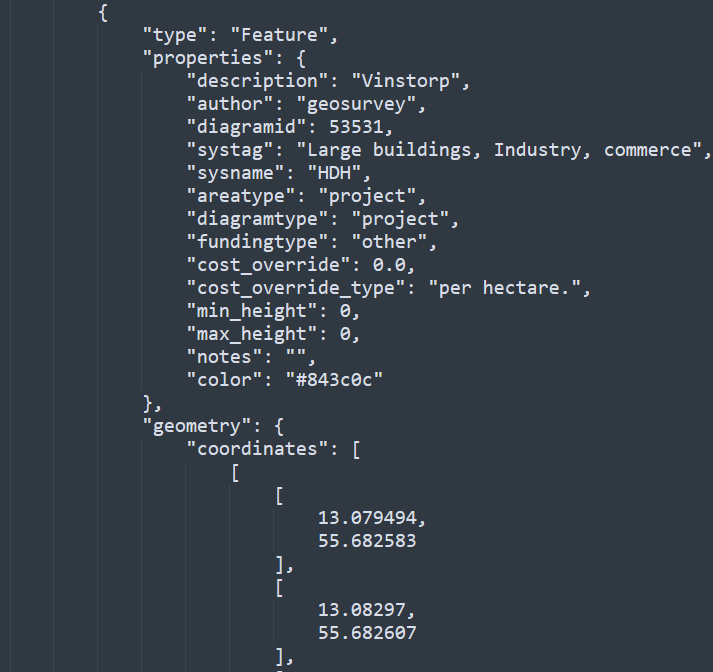
\includegraphics[scale=0.5]{pic1.png}
\label{json}
\end{figure}
Json is an unstructured data type. This format is convenient for transmission and readability, but not for data analysis. Therefore, in order to simplify the process of analysing the two designs, data pre-processing methods are performed on these two JSON files.




\subsection*{Data Pre-processing and EDA}
The main objectives for pre-processing stage is converting JSON (unstructured) data to structured format and finding the underlying metadata. Python is used for reading and manipulating the JSON files of the two designs to extract the metadata. With the aid of library \emph{json}, the two GEOJSON files can be converted to dictionaries in Python. After that, by investigating the data, several rudimentary rules can be found:
\par
(1) Both of the JSON files share the same hierarchical structure.
\par
(2) The structure can be simplified to two layers and the outer layer of each JSON is a list, which contains multiple objects.
\par
(3) The objects in inner layer also share the similar structures and attributes.
\par
A design consists of several entities, such as a site for housing, a place for building a park or an express way, which can be mapped to the objects in the inner layer of JSON data. Meanwhile, the detailed information of each entity is corresponded to the values of attributes of each object. It can be seen that understanding the relationship between GEOJSON data and its physical meaning can facilitate the process of data transforming and metadata retrieving.
\par
The next step is to investigate the attributes of each entity. First, it is obvious that the attributes can be divided into numerical and textual attributes. The numerical attributes define the geometric feature of the entity while the textual attributes indicate the label, description and annotation of the design.
\par
For numerical attributes, the first attribute is ID, which is the identifier of each entities. The most important feature is geographical coordinates, which determines the location of an entity. Some secondary features like area, length can be derived from this attribute. Other attributes like minimum/maximum height and cost override are all the same amongst the entities. Thus, those features were reduced. The last attribute is colour and it can only influence the readability of the images of a design generated by GEOJSON tool but has no contribute to the semantic of the design. As a result, attribute color was also erased.
\par
For textual attributes, the first useful one is type. Attribute type can be only set to ``Polygon" and ``LineString", which indicates that whether the entity is of a closed figure or line. Different kinds of shapes also require different methods for manipulating coordinates. The second attribute is description. This feature is important since it tells the semantic of each entity, for example, an entity with description ``Bike highway" can be directly understood as a kind of road exclusively for bicycles. Another attribute is sysname, which assigns each entity with a geodesignhub built-in label. The value of this attribute can only be ``Large buildings, Industry, commerce", ``Small buildings, low density housing", ``Agriculture, Forestry" or ``Roads, transport". It is attribute sysname that has divided the entities into four categories roughly. 
\par
After sorting numerical and textual features, the metadata can be obtained and Table \ref{tab:metadata} illustrates the attributes that will be used and their comments.
\begin{table}[H]
\centering
\caption{Metadata}
\label{tab:metadata}
\begin{tabular}{|c|c|c|}
\hline
NAME & TYPE & COMMENTS \\ \hline
id & INT & The identifier \\ \hline
coordinate & (FLOAT, FLOAT) & Geographical location of a vertex \\ \hline
description & TEXT & Description of each entity \\ \hline
sysname & TEXT & Can only be four values. \\ \hline
\end{tabular}
\end{table}
After obtaining metadata from the two designs of urban planning, the manipulation against the data can be executed under the guidance of metadata.
\subsection*{Taxonomy Similarity}
The definition of taxonomy is different words for the same idea, and the similarity of taxonomy is the degree to which textual attributes are similar. A very direct example is that a place for ``school" and a site that is projected to be a ``campus" can be naturally grouped together. The reason is that both of them represents the same idea. Although the two schools may be situated in very different places with different area, they both stand for education institutes and are obviously not identical to places with other ideas like ``industrial plants".
\par
It can be found that finding taxonomy similarity mainly focuses on the description, comments or labels of each figure in the designs and neglects other geometric attributes. That is, the textual attributes in the design is the key for defining taxonomy similarity and therefore, natural language processing (NLP) and text mining methodology can be exploited for obtaining similarity of taxonomy.
\par
From the perspective of text mining, it can be seen that obtaining similarity of taxonomy with regard to textual information is to gather the text with the same meaning into groups, which can be also regraded as finding synonyms. In other words, the problem of finding latent taxonomy similarity in the two designs can be solved by computing the similarity of the textual attributes of each design using NLP algorithm.
\par
Since the textual information of each entity in the designs are stored in attribute Description and hence, the description of each figure is utilised for finding taxonomy similarity using NLP approaches. The core idea for finding taxonomy similarity between descriptions is to convert them into word vectors and thereby the distance between the vectors can be computed, where the distance is directly correlated to taxonomy similarity.
\par
In terms of the method of embedding descriptions into vectors, Global Vectors for Word Representation algorithm (GloVe) is adopted. GloVe is an unsupervised learning method based on word count and overall statistics, which can capture the latent analogy and synonym between words \cite{pennington2014glove}. After obtaining word vectors, the description can be embedded into a vector by adding the vector of its words. The following formula shows the process of embedding description into vectors:
\begin{equation}
    {\rm vec}(d)=\sum_{i=1}^{n}{\rm vec}(w_i)
\end{equation}
where $d$ is a description of a figure and it is composed by words $w_1,w_2,...,w_n$.
\par
For the metric of distance between vectors, the cosine similarity is used, which can expressed by the following formula:
\begin{equation}
    s={\rm cos}(\theta)=\frac{|v_1\cdot v_2|}{||v_1||||v_2||}
\end{equation}
where $s$ is similarity and $v_1$,$v_2$ are the vectors for the two descriptions. The value of cosine similarity is corresponding to the taxonomy similarity and if the value is closer to 1, then the two descriptions are very similar, otherwise, they hardly have the same idea. 
\par
By inputting the textual data of the given GEOJSON files, the taxonomy similarity can be visualised by the following heat map, which is displyaed in Figure \ref{heat}.
\begin{figure}[H]
\caption{Heat Map of Pairwise Similarity}
\centering
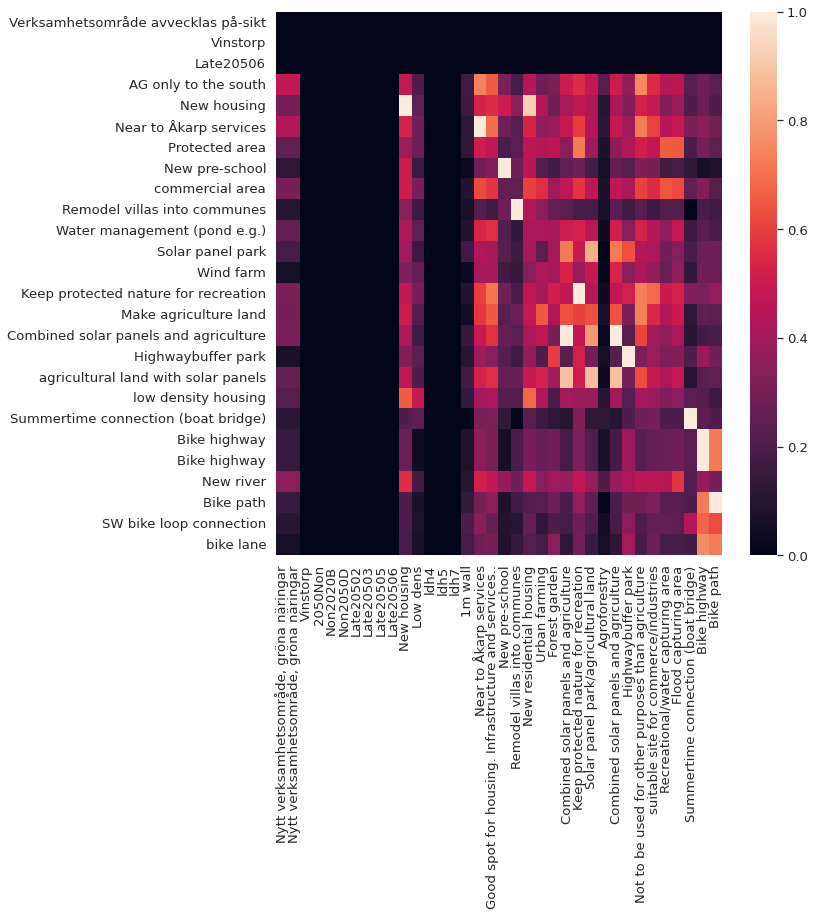
\includegraphics[scale=0.45]{heat.png}
\label{heat}
\end{figure}
\par
It can be found that the designs with the same descriptions definitely feature maximum similarity of taxonomy, for example, both of the design have an entity with description ``New Housing" and the cosine similarity of the two entities is 1. And the descriptions with similar meanings also achieves high similarity like ``Bike Lane" and ``Bike Path". Besides, the designs with irrelevant textual attributes, such as ``New River" and ``Bike Highway", display less similarity score, which is also not out of expectation in real world. 
\subsection*{Topology Similarity}
In addition to the textual attributes, the main difference between the designs exists in the geometric attributes. The main geometric attribute of the data is the coordinates attribute. Coordinates are the set of latitude and longitude of multiple vertices.

Topological similarity is defined as the similarity of different geometry for the same place. In practical planning work, due to various factors, entities are often designed as irregular polygons. Therefore, a comparison of the similarity of entities in geometry should focus on the ratio of the overlapping area of the same places in the two scenarios to the total area of the planned site. The following part of this section focuses the derivation and presentation of the algorithm on polygons.

The main challenge of this part of the work is to derive a method for calculating the area of a polygon when the coordinates of the vertices of the polygon are given. The derivation starts with the simplest polygon, the triangle, and is then extended for calculating the area that can be applied to arbitrary polygons.

Calculation using matrix determinants is at the heart of this part of the algorithm. The geometric meaning of a matrix determinant is the directed area of a parallelogram with two vectors as a set of neighbors. (Directed in the sense that the area is positive if the second vector is rotated 0 to 180° counterclockwise with respect to the first vector, and negative if the second vector is rotated 0 to 180° clockwise with respect to the first vector.)

Suppose there is a general triangle and a rectangular coordinate system is set up to place this triangle in it. First, it is assumed that the origin $O$ lies inside the triangle (the case where the origin is outside the triangle will be described later).

\begin{figure}[H]
\caption{$\triangle ABC$ in The Coordinate System}
\centering
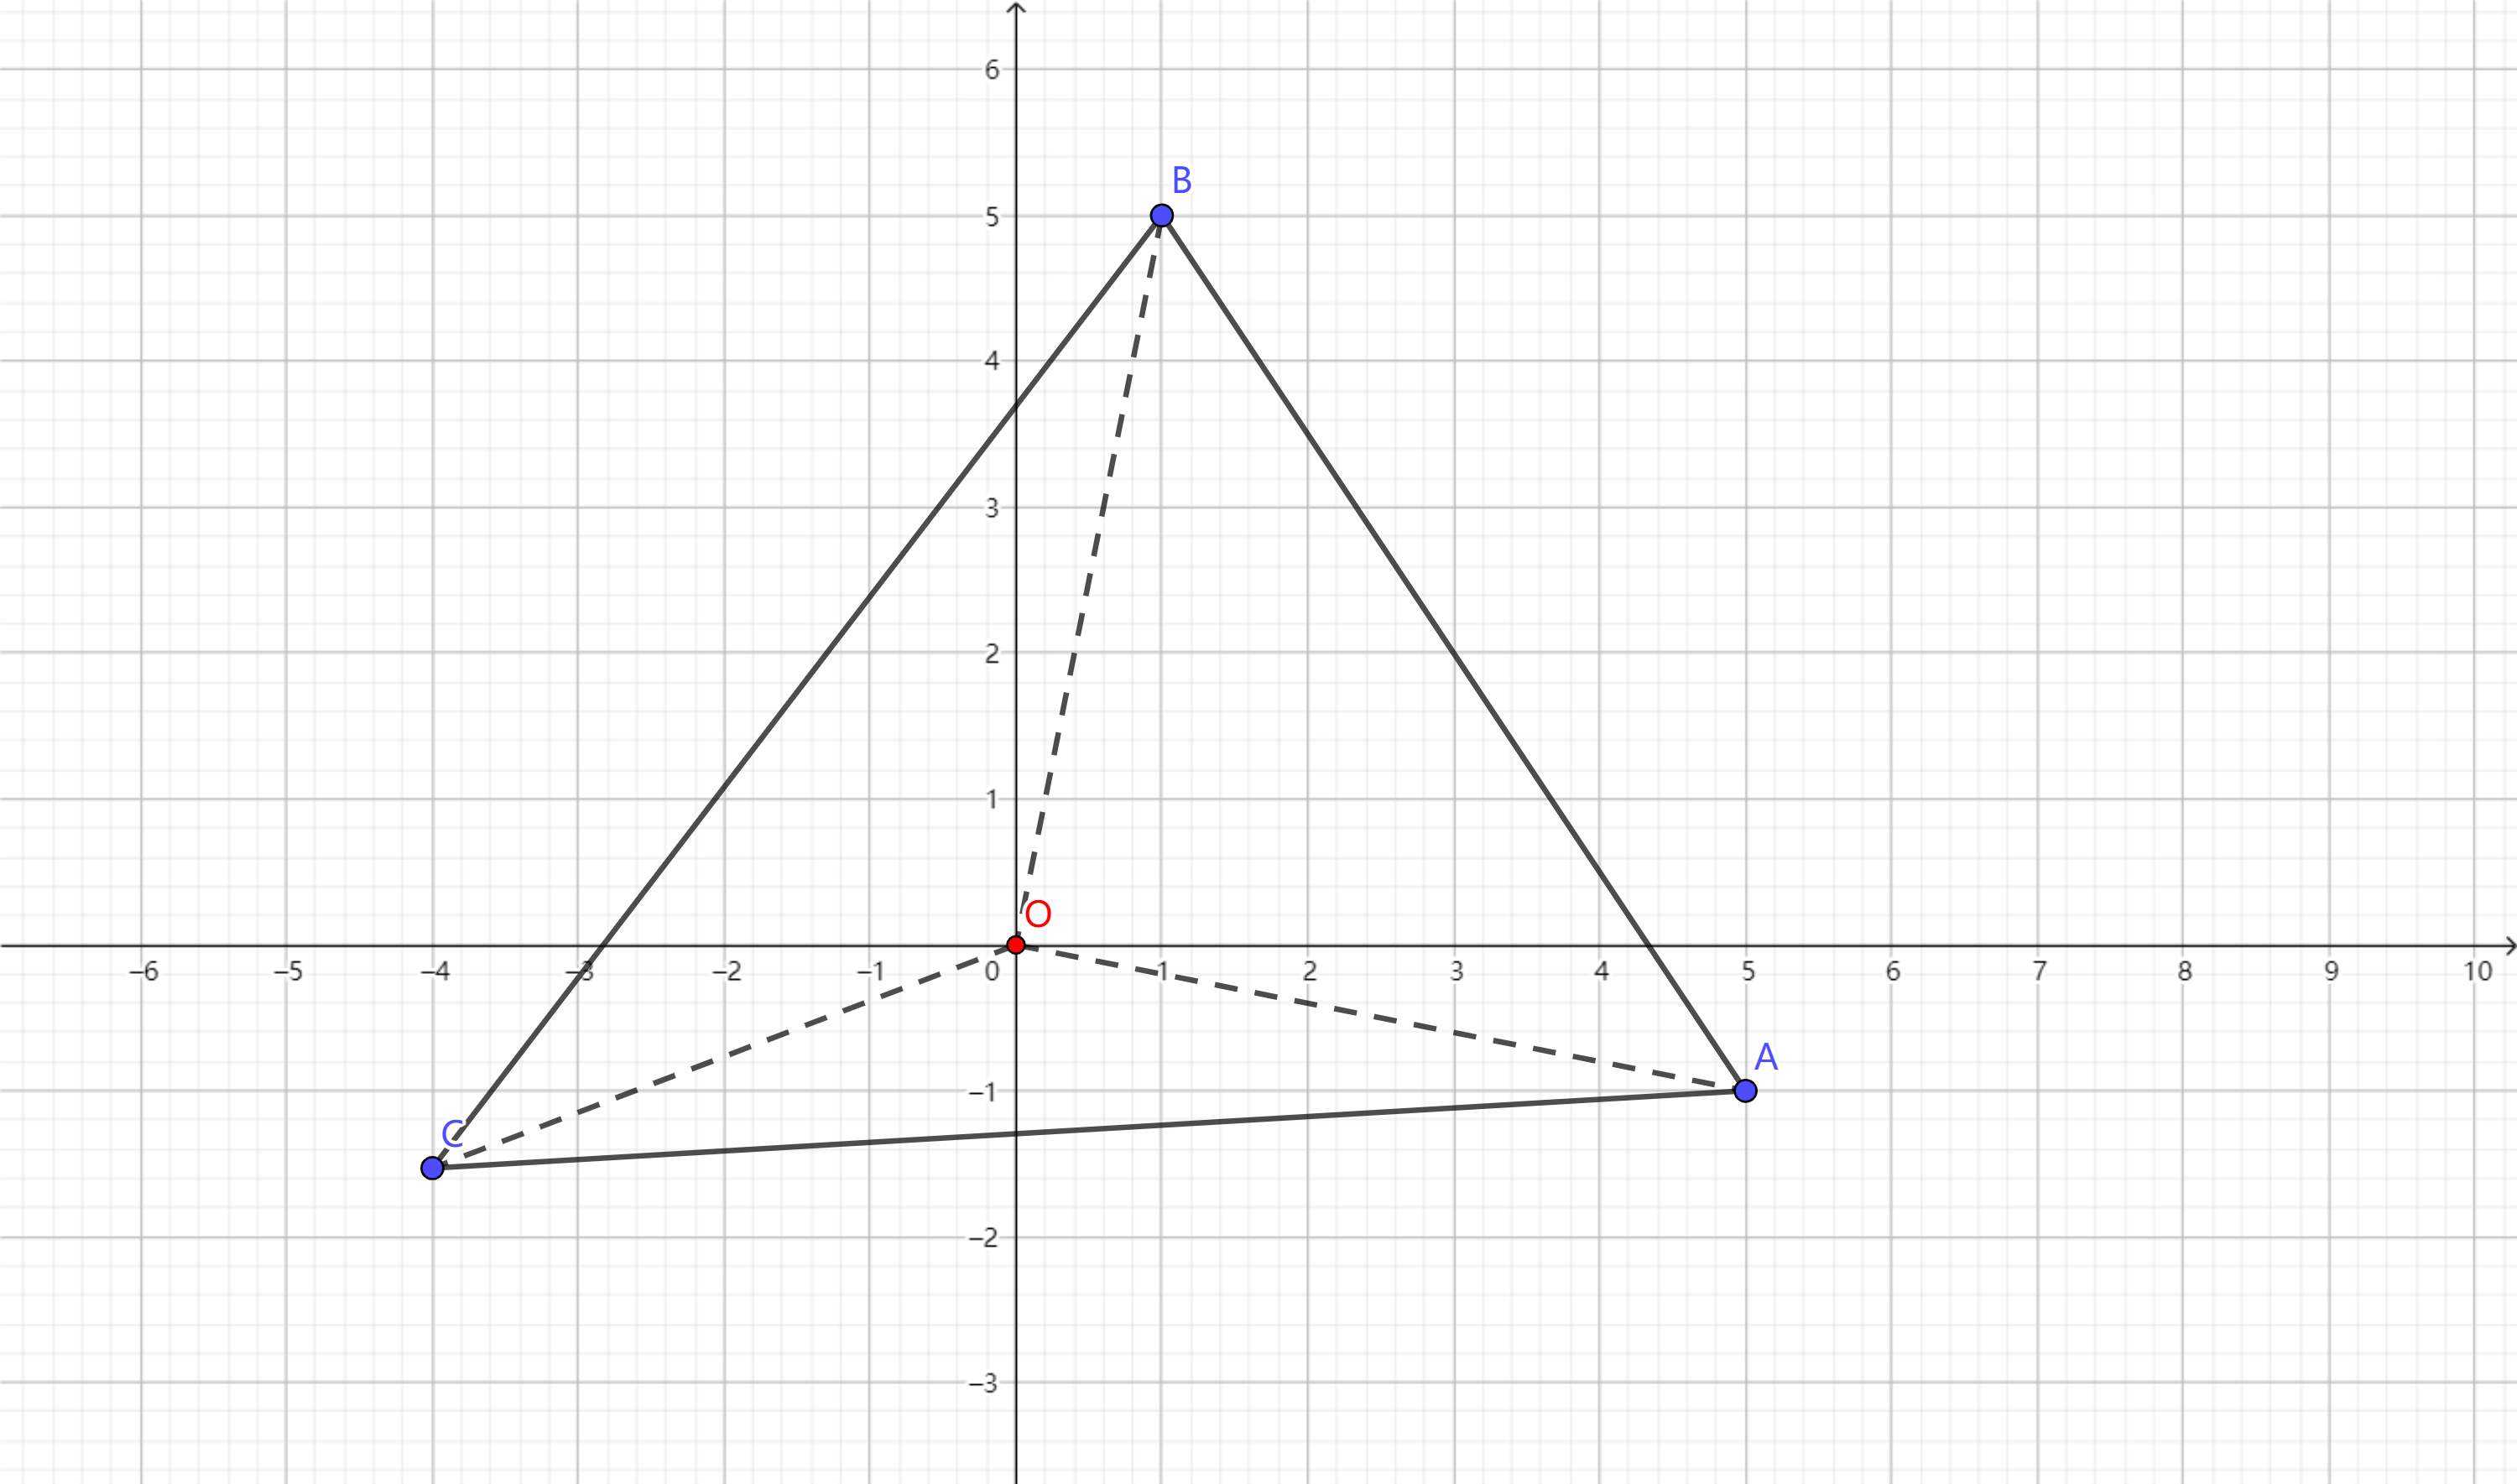
\includegraphics[scale=0.5]{pic2.png}
\label{topo1}
\end{figure}

As shown in Figure \ref{topo1}, $S_{\triangle ABC}$ is split into $S_{\triangle AOB}$, $S_{\triangle AOC}$ and $S_{\triangle BOC}$.   $S_{\triangle AOB}$ is calculated first.

\begin{figure}[H]
\caption{Flipping $\triangle ABC$}
\centering
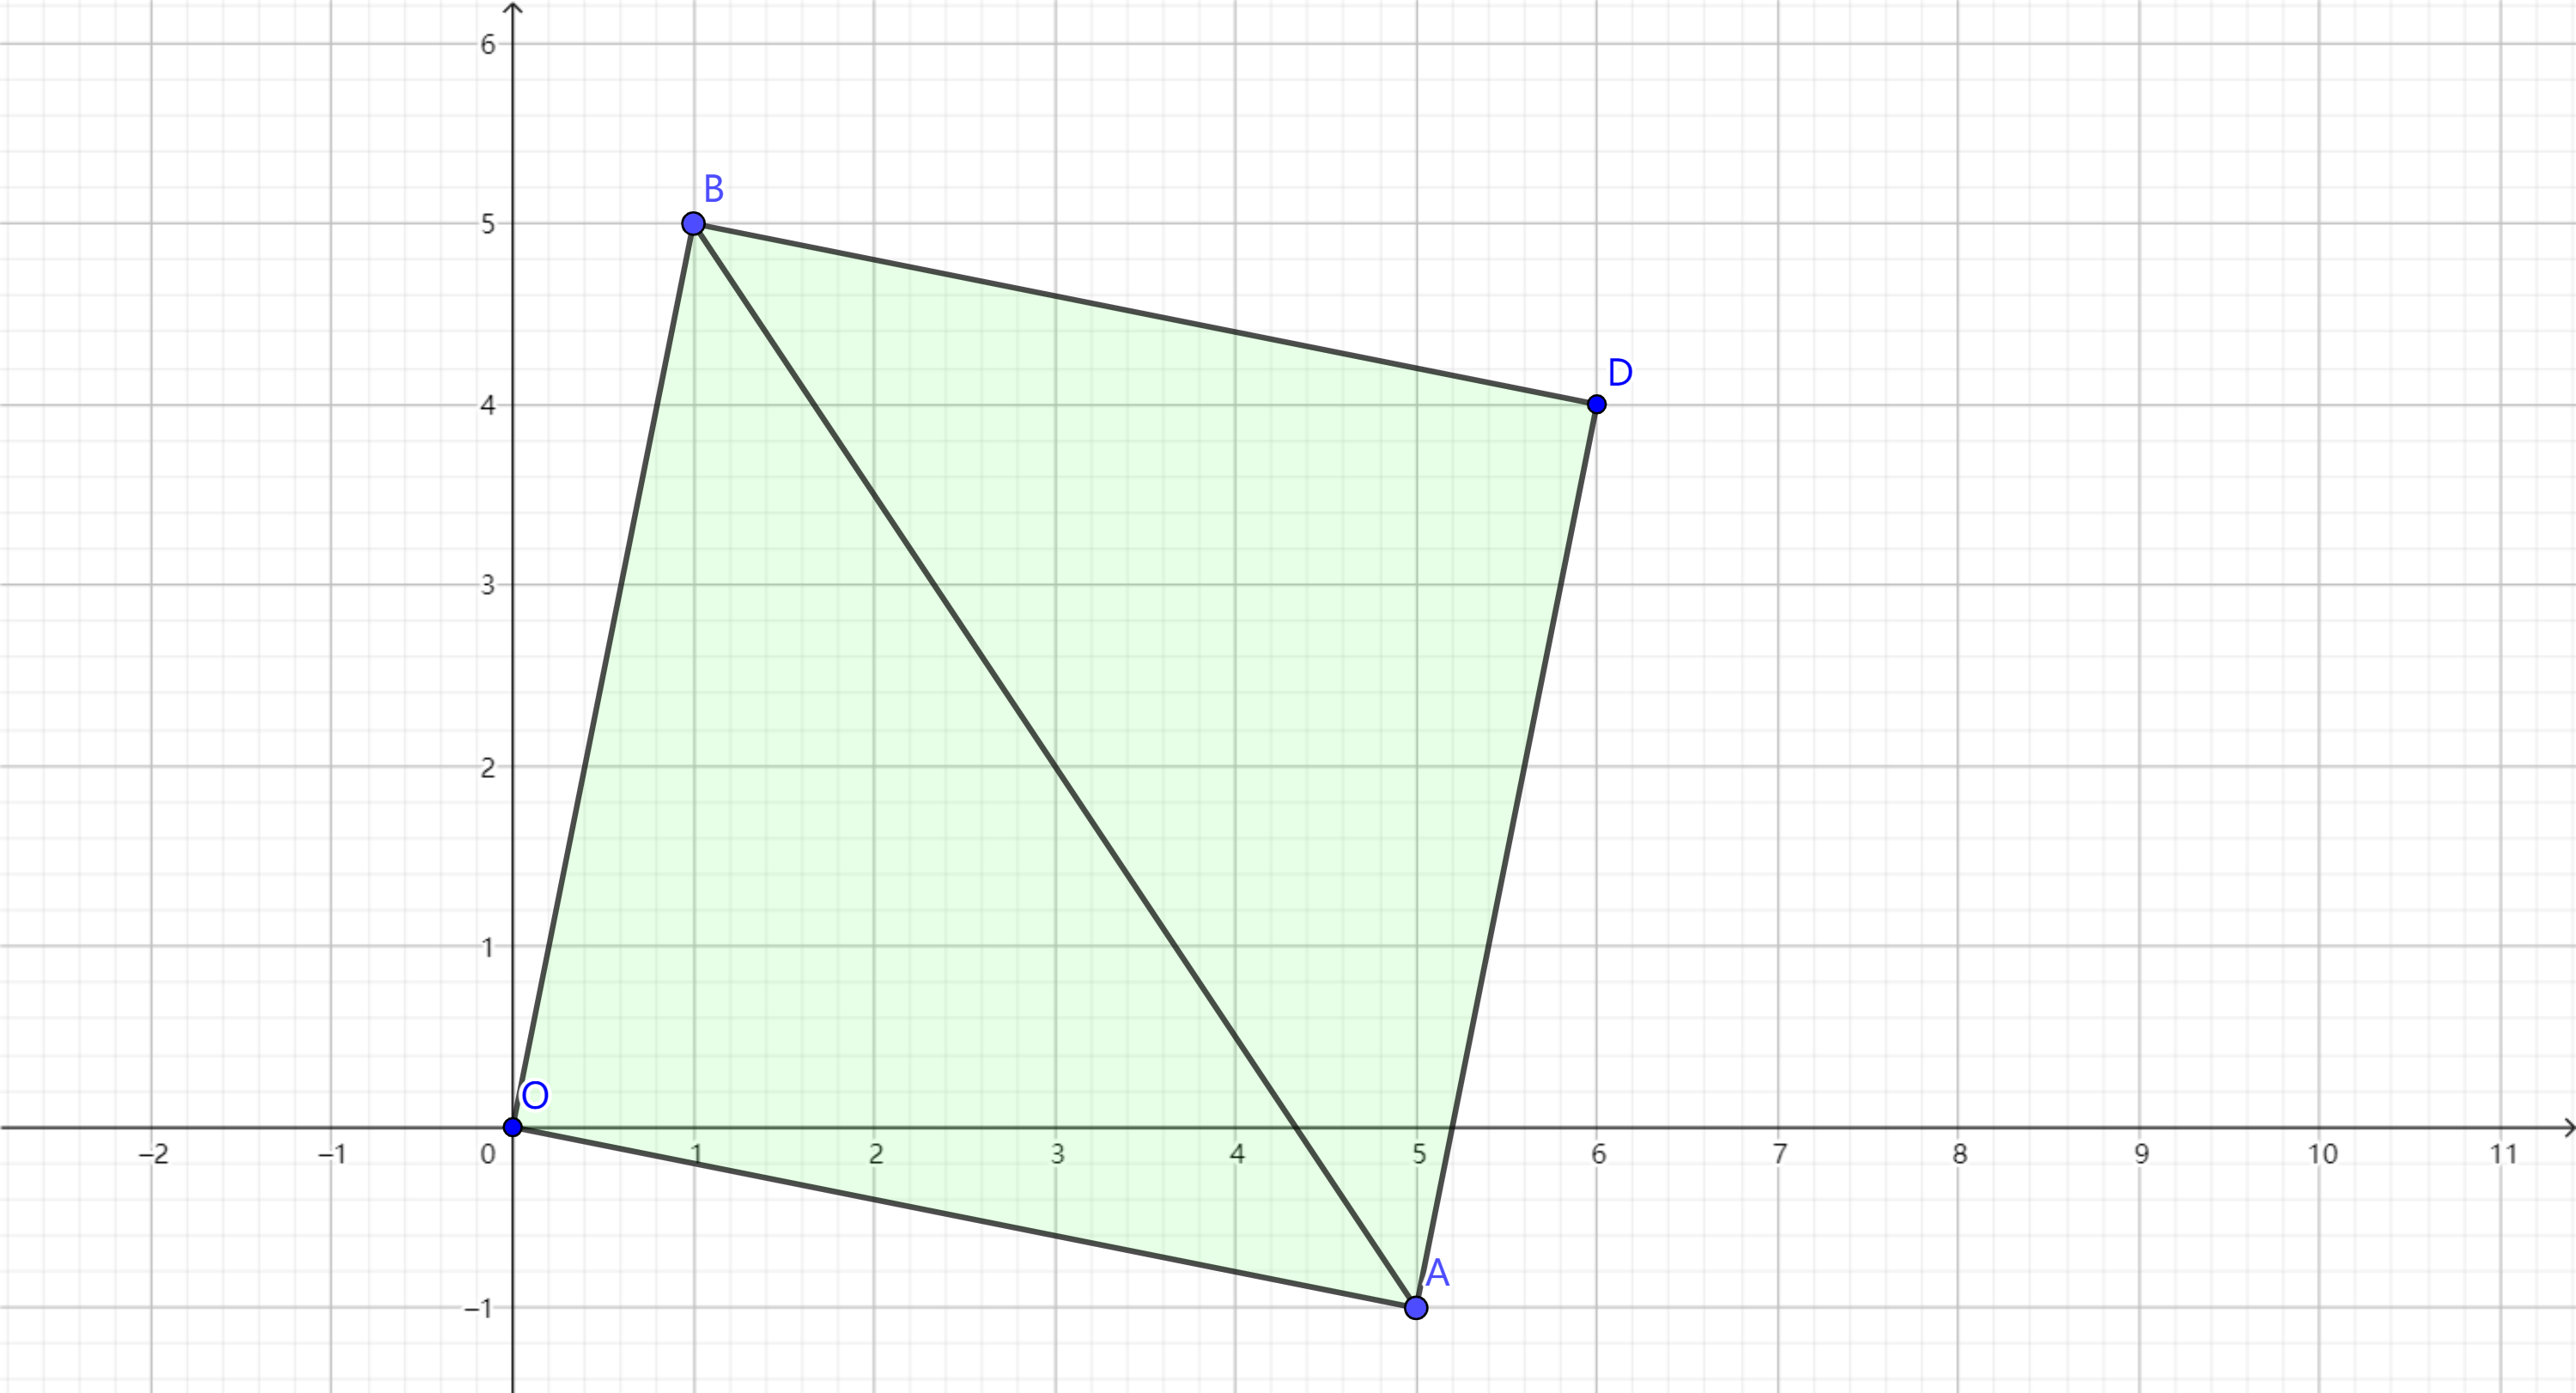
\includegraphics[scale=0.5]{pic3.png}
\label{topo2}
\end{figure}

Taking $AB$ as the axis of symmetry and flipping $S_{\triangle ABC}$ (shown in Figure \ref{topo2}), the area of parallelogram $AOBD$ can be expressed in matrix determinant as:

\begin{equation}
\begin{split}
S_{\parallelogram AOBD}=\begin{vmatrix}
  x_{A} &x_{B}  \\
  y_{A} &y_{B} 
\end{vmatrix}
\end{split}
\end{equation}

So that the area of $\triangle AOB$ is half of it;

\begin{equation}
\begin{split}
S_{\triangle ABC} =\frac{\begin{vmatrix}
  x_{A} &x_{B}  \\
  y_{A} &y_{B} 
\end{vmatrix}}{2}=\frac{x_{A}y_{B}-x_{B}y_{A}}{2}   
\end{split}
\end{equation}

The area of $\triangle AOC$ and $\triangle BOC$ is calculated in the same way, and then:

\begin{equation}
\begin{split}
S_{\triangle ABC}
&=S_{\triangle AOB}+S_{\triangle BOC}+S_{\triangle COA}\\
&=\frac{\begin{vmatrix}
  x_{A} &x_{B}  \\
  y_{A} &y_{B} 
\end{vmatrix}+\begin{vmatrix}
  x_{B}& x_{C}\\
  y_{B}&y_{C}
\end{vmatrix}+\begin{vmatrix}
  x_{C}&x_{A} \\
  y_{C}&y_{A}
\end{vmatrix}}{2}\\
&=\frac{(x_{A}y_{B}-x_{B}y_{A})+(x_{B}y_{C}-x_{C}y_{B}) +(x_{C}y_{A}-x_{A}y_{C})  }{2}\\
&=\frac{(x_{A}y_{B}+x_{B}y_{C}+x_{C}y_{A})-(x_{B}y_{A}+x_{C}y_{B}+x_{A}y_{C})}{2}
\end{split}
\end{equation}

When the origin $O$ is outside $\triangle ABC$, there will be a sub-triangle whose area determinant is negative, so the formula still applies when brought into $\triangle ABC$.

This area calculation method can be extended to any polygon. Given an arbitrary polygon, it can be divided into multiple triangles. The area of the polygon can be obtained by summing the areas of these triangles using the matrix determinant.
The formula is:
\begin{equation}
\begin{split}
S_{Polygon}= \left | \frac{(x_{1}y_{2} +x_{2}y_{3}+...+x_{n}y_{1} )-(x_{1}y_{n} +x_{2}y_{1}+...+x_{n}y_{n-1})}{2}  \right | 
\end{split}
\end{equation}

where $i=1,2,...,n$ denotes the $i$-th point and ($x_{i}$, $y_{i}$) denotes the coordinates of the $i$-th point.

After discussing how to calculate the area of a polygon using vertex coordinates, the next step is to discuss the calculation of topological similarity.

Suppose there are two planning designs to compare, $D_1$ and $D_2$, and the sites they are planning to develop are called Site 1 and Site 2, with area $S_1$ and $S_2$ respectively, and the site planned to be developed in both schemes is called Overlapping Site, which has an area of $S_3$.

It should be noted that the area $S_3$ of the overlapping area between the two proposals requires a solution algorithm to be devised. It is a typical problem of solving for the intersection of polygons and has some computational complexity. The algorithm is designed to calculate the intersection of polygons as solution. Given the complexity of the proof process of the algorithm\cite{bib10}, the concepts required by the algorithm and some properties used by the algorithm are directly given here.

The concepts used in the algorithm include:

1. $\partial A$: The set of sides of a polygon $A$, or the set of points on the boundary of $A$;

2. $P\downarrow$: A vertical downward ray through point $P$;

3. <: Less-than comparator for point, $P < Q \Leftrightarrow (P_x < Q_x )\vee (P_x =Q_x \wedge  P_y < Q_y)$;

4. $P_{x},P_{y}$: Horizontal and vertical coordinates of $P$;

5. $e, s$: sides;

6. $Lp(e)$: the left endpoint of $e$, i.e. the smaller of the two endpoints of $e$;

7. $Rp(e)$: the right endpoint of $e$, i.e. the bigger of the two endpoints of $e$;

8. $I(e)$: The set of points within $e$ (points on $e$ other than endpoints);

9. $C(P , \partial A) $: the set of edges of $A$ with intersection with $P\downarrow$ and whose right endpoint is not on $P\downarrow$;

10. $s_{1}\;\mathop  > \limits^P  \;s_{2}$: Comparison of the sides $s_{1}$ , $s_{2}$ on the perpendicular line $x = P_x$ through the point $P$, i.e. $s_{1} \; \mathop  > \limits^P \; s_{2} \; (Q_1 >Q_2)\vee  (Q_{1}  =Q_{2}  \wedge K(s_{1})  >K(s_{2}) )$, where Points $Q_{1}$ , $Q_{2}$ denote the intersection of sides $s_{1}$ , $s_{2}$ with the vertical line through point $P$, and $K(s_{1})$ , $K(s_{2})$ denote the slopes of $s_{1}$ , $s_{2}$ respectively;  

11. $max(C(P , \partial A))$: the largest edge in $C(P , \partial A)$ at point $P$.

Theorems and properties used in the algorithm include:

1. For any edge of polygon $A$, let $P$ be the interior point of $e$. If $C(P , \partial A)$ has an odd number of edges, then $e$ is said to be an odd edge of $A$, abbreviated as $+e$, otherwise $e$ is said to be an even edge of $A$, abbreviated as $-e$.

2. For any two edges $s_{1}, s_{2}\in  C(P,\partial A)$, $s_{1}$ , $s_{2}$ have different parity in $A$ if $s_{2}$ is the largest edge smaller than $s_{1}$ at point $P$ , i.e. $s_{1}$ >P $s_{2}$ , and there is no edge $e\in  C(P,\partial A)$ such that $s_{1}$ >P e , e >P $s_{2}$ hold simultaneously.

3. For any point P not on the boundary of polygon A, if the largest side of the perpendicular downward ray made through the point P which intersects polygon A is an even side, or does not intersect any side of A, then P is in the outer domain of polygon A, and vice versa; if the largest side of the ray which intersects A is an odd side, then P is in the inner domain of polygon A, and vice versa.

4. interior edge: all interior points of e lie in the interior domain of A. $P , \; P\in  I(e)\; P \in  I (A)$.

5. exterior edge: all interior points of e lie in the exterior domain of A. $P , \; P\in  I(e)\; P \in  E (A)$.

6. Overlapping sides: $s , s \in  A , P , P \in  e \ P \in  s$.

7. Simple edges: interior edges, exterior edges, overlapping edges.

8. Complex edges: any other edges that are not simple edges.

General flow of the algorithm:

1. While scanning the plane, the intersection points (including tangent points) of $A$ , $B$ are calculated, and the complex edges are decomposed into simple edges. Meanwhile, the parity of the edges of $A$ , $B$ and their topology types are determined according to Theorems 1 and 2 , and recorded in the data structure;

2. For the specific computational characteristics of the intersection of polygons, edge tracing is performed according to the theorem, and the intermediate polygons forming $A \cap  B$ are output;

3. Construct the border of each intermediate polygon in turn, and determine the direction of the intermediate polygon. Determine whether it is a hole or an external polygon according to the theorems and properties.

4. Determine the containment relationship between the hole border and the outer polygon border to determine which outer polygon the hole belongs to, and then determine $A \cap  B$.

Then the topological similarity($TPL$) formula for these two planning designs is:
\begin{equation}
\begin{split}
TPL=\frac{2*S_{3} }{S_{1}+S_{2}  } 
\end{split}
\end{equation}


\subsection*{Geography and Conceptual Similarity}
In the sections above, the concepts and implementation of topology and taxonomy were introduced. Taxonomy gives a specific meaning to the concepts of the ``same idea": when comparing the properties of two regions within the two proposals, if these two regions have high taxonomy similarity, they have the ``same idea". About nine types of taxonomy participates in the taxonomy similarity-examination process. Topology similarity actually explores the degree of overlap between the two regions defined by the two proposals. Because both of the proposals are actually based on the same latitude and longitude, and they aims at exploring the planning differences for the same block, calculating the area of the overlapping area provides the basis for later explorations. However, the overlapping region is easy to understand conceptually, but complex to implement. To do this, a sophisticated algorithm was devised to calculate the overlapping area. Geography and conceptual similarity uses the definition of topology and taxonomy to explore the special properties in the regions of conceptually identical or overlapping parts respectively.
\subsubsection*{Geography Similarity}
Geography similarity measures the degree of idea replication in different places. In other words, it measures the ratio of area with the same idea to the total area. It calculates the extent to which the regions with the same idea overlap in the two proposals. Picture \ref{geo1} shows a simple example of the calculation of the geography similarity. 

\begin{figure}[H]
\caption{An Example of Calculating Geometry Similarity}
\centering
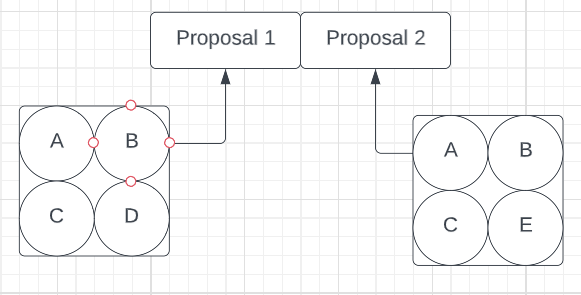
\includegraphics[scale=0.7]{Geo-1.png}
\label{geo1}
\end{figure}

The two large squares represents all regions of the two proposals, while the four circles stands for regions of different ideas. The two designs share a common type of region $A,B,C$, but occupies the different regions $D$ or $E$. The area of the five regions are shown in Table \ref{geo3}.

\begin{table}[H]
\centering
\caption{The area for the five regions}
\label{geo3}
\begin{tabular}{|c|c|c|c|c|c|c|}
\hline
       & Total Area & Area for $A$ & Area for $B$ & Area for $C$ & Area for $D$ & Area for $E$ \\ \hline
Proposal 1 &    $S_{proposal1}$       &     $S_{A1}$       &    $S_{B1}$          &       $S_{C1}$       &           $S_{D1}$   &    $S_{E1}$          \\ \hline
Proposal 2 &   $S_{proposal2}$         &    $S_{A2}$        &     $S_{B2}$       &   $S_{C2}$     &       $S_{D2}$     &    $S_{E2}$        \\ \hline
\end{tabular}
\end{table}
From the formula of calculating the overlapping area between two proposals in the previous section, the topology similarity of the area of the same idea $A$ can be calculated as:
\begin{equation}
 G(A) = \frac{2S_{Overlapping(A)}}{S_{A1}+S_{A2}}   
\end{equation}
Then, the overlapping area between the two proposals can be calculated as:
\begin{equation}
S_{Overlapping(A)}=min(S_{A1},S_{A2})
\end{equation}

In this case, the geometry property of a certain idea can be directly calculated as shown in Formula \ref{cao1}. However, calculating the geometry similarity of the proposals is to calculate the weighted average of individual ideas, so the entire procedure can be expressed as:
\begin{equation}
\label{cao1}
    \begin{split}
        G(A,B,C,D,E) & =  {\frac{2S_{Overlapping(A)}}{S_{A1}+S_{A2}}} \times {\frac{S_{A1}+S_{A2}}{S_{proposal1}+S_{proposal2}}} +
        {\frac{2S_{Overlapping(B)}}{S_{B1}+S_{B2}}} \times {\frac{S_{B1}+S_{B2}}{S_{proposal1}+S_{proposal2}}}\\
        & + {\frac{2S_{Overlapping(C)}}{S_{C1}+S_{C2}}} \times {\frac{S_{C1}+S_{C2}}{S_{proposal1}+S_{proposal2}}} +
        {\frac{2S_{Overlapping(D)}}{S_{D1}+S_{D2}}} \times {\frac{S_{D1}+S_{D2}}{S_{proposal1}+S_{proposal2}}}\\
        &+ {\frac{2S_{Overlapping(E)}}{S_{E1}+S_{E2}}} \times {\frac{S_{E1}+S_{E2}}{S_{proposal1}+S_{proposal2}}}\\
        & = \frac{2(Overlapping(A)+Overlapping(B)+Overlapping(C)+Overlapping(D)+Overlapping(E))}{S_{proposal1}+S_{proposal2}}
    \end{split}
\end{equation}
In this project, 8 categories of regions are included in the two proposals, so the final formula of geometry similarity formula of the two proposals can be calculated as: 
\begin{equation}
C = \{A,B,C,D,E,F,G,H\}
\end{equation}
Using the previous Topology calculation for the area, the total area for the two proposals and the area of each category area can be derived separately.
\begin{equation}
\begin{split}
S_1=\{S_{proposal1},S_{A1},S_{B1},S_{C1},S_{D1},S_{E1},S_{F1},S_{G1},S_{H1}\}\\ 
S_2=\{S_{proposal2},S_{A2},S_{B2},S_{C2},S_{D2},S_{E2},S_{F2},S_{G2},S_{H2}\}
\end{split}
\end{equation}

The geometry for a single them can be expressed as:
\begin{equation}
G_{C_{i}}=min(S_{C_{i1}},S_{C_{i2}}) \;  C_i \in C 
\end{equation}
The geometry for the two files can be expressed as
\begin{equation}
Geo=G(A,B,C,D,E,F,G,H) =  \sum\limits_{{C_i} \in C} {\min ({S_{{C_{i1}}}},{S_{{C_{i2}}}})} 
\end{equation}

\subsubsection*{Conceptual Similarity}
Conceptual similarity determines the different ideas for the same place. In other words, it decides how many ideas exist in the overlapping area of the two proposals. Picture \ref{7777} shows a basic example for the conceptual similarity calculation process.
\begin{figure}[H]
\caption{An Example of Calculating Conceptual Similarity}
\centering
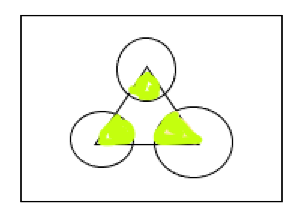
\includegraphics[scale=0.7]{777777.png}
\label{7777}
\end{figure}
The square area represents an area for exploring conceptual similarity. In the actual situation, the same part of region can be chosen in the two proposals to explore this property, with area $S_{total}$. The circular region are from the proposal 1, with area $S_{proposal1}$. The triangular region are from the proposal 2, with area $S_{proposal2}$. The region with green shadow represents the overlapping place generated by the two proposals, with area $S_{shadow}$.It is worth noting that the definition of Conceptual similarity is also closely related to the overlapping area, so its calculation is still closely related to the calculation of topology similarity.

In the example show in Figure \ref{7777}, there may be multiple ideas in the overlapping sector. For any idea $A$, the coincident regions in the two proposals can be represented as:
$$
S_{overlapping} = min(S_{A1},S_{A2}) 
$$
where $S_{A1}$ and $S_{A2}$ represent the corresponding area of idea $A$ in proposal 1 and 2. if there are only 3 ideas $A$, $B$, $C$, the equation for the conceptual similarity will be
\begin{equation}
    Con = \frac{S_{overlappingA}+S_{overlappingB}+S_{overlappingC}}{S_{total}}
\end{equation}
The results should be extended to real problems. 9 ideas are included in the regions, with representation $A$,$B$,$C$,$D$,$E$,$F$,$G$, so the formulation for the conceptual calculation can be represented as:
\begin{equation}
    Con = \frac{S_{overlappingA}+S_{overlappingB}+S_{overlappingC},+S_{overlappingD},+S_{overlappingE},+S_{overlappingF},+S_{overlappingG}}{S_{total}}
\end{equation}


\section*{Evaluation and Discussion}
\subsubsection*{Taxonomy Similarity}
From the discussion on taxonomy similarity above, it can be found that obtaining this metric should exploit the technique of texting mining, the physical semantic of each entity and some expert knowledge of urban designing. Also, it is required that the metric should be represented as five discrete values from low to high similarity. Hence, the main idea for designing the algorithm is combined with the following discoveries and conclusions:
\par
(1) If the description of both entities are identical, they must be in maximum similarity.
\par
(2) Entities in the same category (have the same value of attribute ``sysname") tend to have more in common since each category usually represents the same place of urban planning.
\par
(3) The similarity of word vectors for descriptions is consecutive and can be mapped to categorised values.
\par
Therefore, a decision-tree-like method has been implemented to compute the similarity of taxonomy and Figure \ref{eva_tax} displays the procedure.
\begin{figure}[H]
\caption{Process of Calculating Taxonomy Similarity}
\centering
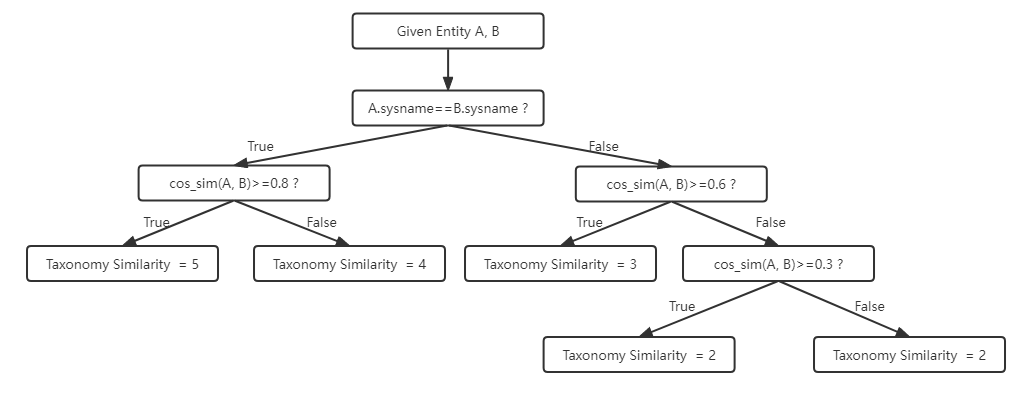
\includegraphics[width=1.0\textwidth]{eva_tax.png}
\label{eva_tax}
\end{figure}
\par
Given the details of computing similarity of taxonomy, the algorithm can be implemented by retrieving the description and category of all entities, generating pairwise similarity of word vectors by texting mining technique and constructing a pseudo decision tree for obtaining the score of taxonomy similarity. By inputting the two given designs, the result of taxonomy similarity with regard to the entities is displayed in Figure \ref{tax_sim} as another heat map.
\begin{figure}[H]
\caption{Heat Map of Visualising Taxonomy Similarity}
\centering
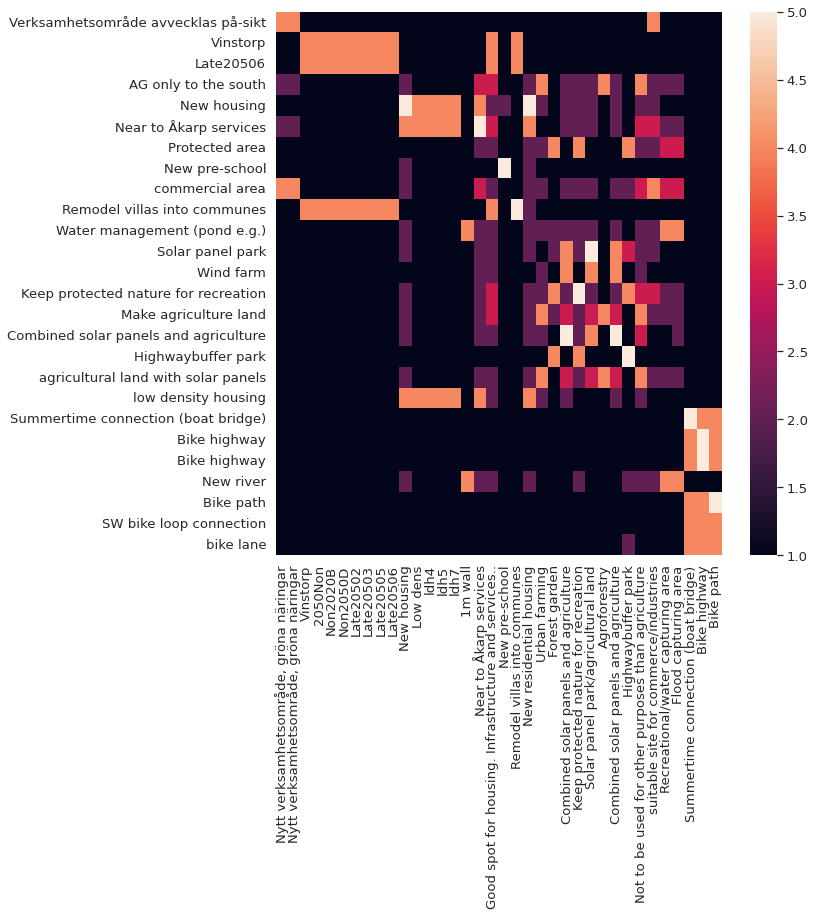
\includegraphics[scale=0.45]{tax_sim.png}
\label{tax_sim}
\end{figure}
\par
From the result, it is obvious that the entities with the same description are in the highest level of taxonomy similarity (Tier 5). The entities in similarity of Tier 4 also demonstrates a significant correlation, for example, ``Bike Path" versus ``Bike Lane" and ``Low Density Housing" versus ``Low Dens". For entities in the medium taxonomy similarity (Tier 3), it can be seen that the descriptions of entities pair may have something in common, for instance, ``Keep Protected Nature for Recreation" and ``Combined Solar Powers And Agriculture" both is relevant to natural resource. The entities in low similarity (Tier 2 or 1) shows low level of relationship and even contrary meanings of description, a typical pair of entities are ``Solar Panel Park" and ``New Housing", where the formal entity is designed as a infrastructure land and the other one is for citizens' living. Thus, it is apparent that this method of finding taxonomy similarity can find similarity of textual attributes and sort them into different hierarchies and the automatic process ensures the time saving of avoiding assessing each piece of textual information by hand. 
\par
As for the limitations, it can be found that some of the entities pairs with zero taxonomy similarity are not true, one reason is that some of them are not written in English like ``Verksamhetsområde avvecklas på-sikt" or some are in abbreviation like ``LDH4" (which is very probably ``Low Density Housing No.4"). Then, these kind of entities cannot be distinguished by its description so that will be set to default value zero. Another improvement can be done is that the entities in the same design tend to have significant similarity like and it can be done by firstly grouping the entities of one design with high relationship into one cluster and comparing the clusters across entities.
\subsubsection*{Evaluation-Topological Similarity}
In the above, the calculation of $TPL$ is described as a measurement of topology similarity are arbitrary, which does not have jumps in values. Therefore, Table \ref{eva_topo} shows the topology similarity between the two proposals into five classes: 

\begin{table}[H]
\centering
\caption{Topological Similarity}
\label{eva_topo}
\begin{tabular}{|c|c|c|c|c|c|c|}
\hline
Topological Similarity & 1 & 2 & 3 & 4 & 5          \\ \hline
$TPL$ & [0, 0.2) &  [0.2, 0.4) & [0.4, 0.6)  & [0.6, 0.8)  &[0.8, 1]   \\ \hline
\end{tabular}
\end{table}

The five tiers (1-5) of topology similarity reflect the meanings of extremely different, hardly similar, moderately similar, very similar and extremely similar.

If the assessed value of topology similarity is 1, then there is little overlap of design proposals in the two planning schemes. The likelihood of this happening in practice is very low. Planners should design proposals to suit the local context and take into account as many constraints and design objectives as possible in their decisions. There should not be such a large difference between schemes in the same context. If this happens, it means that at least one of the two alternatives is extremely unreasonable.

If the assessed value of topological similarity is 5, then the two planning options are almost identical in terms of the choice of development sites. At this point the decision maker should focus on the few differences between the two proposals and make a choice of proposal based on the differences by modelling the values of the indicators after development and conducting a sensitivity analysis. If the two design options can be compared on the basis of high topology similarity, it is safe to conclude that such decision process is rigorous.

Take the comparison between these two proposals as an example. The areas that are developed in the two proposals are shown in yellow and blue in Figure \ref{eva_topo_example}. With this visual presentation, the decision maker is able to get an intuitive impression of the two proposals, but it is difficult to draw intermediate conclusions that are informative. Applying the algorithm of this study, a topology similarity of 66.01\% is calculated, which is defined as the fourth level of similarity: ``very similar", according to the similarity assessment criteria proposed in the previous section.




\begin{figure}[H]
\caption{Topology Similarity of The Example Designs}
\centering
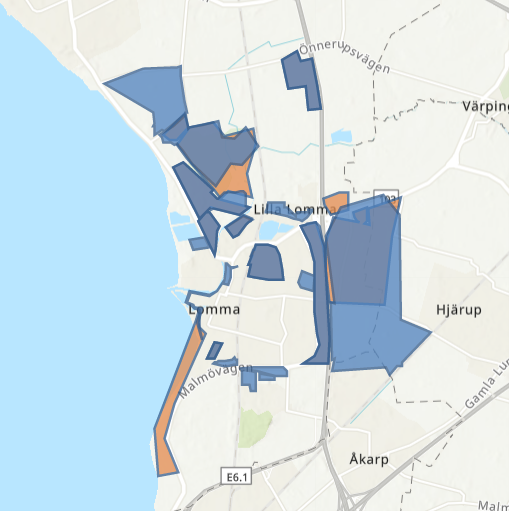
\includegraphics[scale=0.5]{pic4.png}
\label{eva_topo_example}
\end{figure}

\subsubsection*{Geography and Conceptual Similarity}
Geography and Conceptual Similarity criteria are similar to that of the topology, with the same domain. The calculated ratio indicates the geographic nature for the two proposals, which can be seen in Table \ref{tab:my-tablettt} and \ref{tab:my-tableeee}.

\begin{table}[H]
\centering
\caption{Geometry Similarity}
\label{tab:my-tablettt}
\begin{tabular}{|c|c|c|c|c|c|c|}
\hline
Geometry Similarity & 1 & 2 & 3 & 4 & 5          \\ \hline
GEO & [0, 0.2) &  [0.2, 0.4) & [0.4, 0.6)  & [0.6, 0.8)  &[0.8, 1]   \\ \hline
\end{tabular}
\end{table}
\begin{table}[H]
\centering
\caption{Conceptual Similarity}
\label{tab:my-tableeee}
\begin{tabular}{|c|c|c|c|c|c|c|}
\hline
Conceptual Similarity & 1 & 2 & 3 & 4 & 5          \\ \hline
Con & [0, 0.2) &  [0.2, 0.4) & [0.4, 0.6)  & [0.6, 0.8)  &[0.8, 1]   \\ \hline
\end{tabular}
\end{table}
Geography reflects the proportion of areas with the same usage meaning to the overall area. In other words, what this metric wants to see is how the two schemes overlap in design. If the value of Geography similarity is relatively high, it means that the two proposals are relatively similar in design. The specific results are shown in Figure \ref{yes}. It represents the area of overlapping with the same idea. Brown and dark blue each represent an idea. The larger the area of these parts, the closer the Geometry result is to 1


Conceptual means the opposite, it is used to show the diversity of an area. Its judgments are also assigned according to ratings.In general, if the Conceptual value is larger, it indicates that the two program designs are diverse. Here, we plan to separate the overlapping areas to facilitate our analysis of each area and also to analyze the document as a whole. If a small area has a relatively high Conceptual value, it means that the area has some diversity. In other words, the area can have multiple uses in the design. If the value is higher for the whole problem piece, it means that there is some divergence in the design of the two solutions and the similarity is not obvious



\begin{figure}[H]
\caption{The picture for the results}
\centering
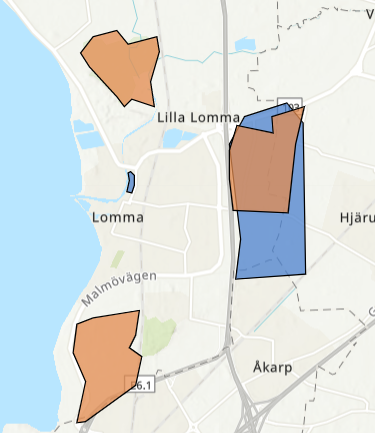
\includegraphics[scale=0.7]{yes.png}
\label{yes}
\end{figure}




\section*{Conclusion}
In this article, a method for assessing the similarity of two GEOJSON designs is created, implemented and evaluated. Firstly, the structure and feature of GEOJSON data is obtained and it can be found that GEOJSON data is of unstructured data type. In order to facilitate the subsequent process of manipulating and analysing data, GEOJSON data is required to be converted to structured format. Python library is utilised to perform data transformation. After attaining data in structured type, the metadata of the dataset can be retrieved, which summarises the attributes to be examined and their information. The next stage is proposing methodology for calculating similarity and the similarity of the two designs are concentrated on four metrics: taxonomy, topology, geography and conceptual. Algorithm and workflow are introduced with regard to each metric, which is rated in five tiers. Taxonomy similarity is completely based on the analysis on textual attributes of the designs and texting mining method is adopted. The key of finding taxonomy similarity is to compute word vectors of descriptions and their cosine similarity. By integrating the semantic of entities themselves and similarity of word vectors, a decision-tree-like algorithm can be performed. Topology similarity is to investigate the latent relationship in numerical attribute and the key point is to computing overlapping area. The pseudo code of the algorithm for solving overlapping area based on the coordinates of the vertices of polygon is given and it is used to obtaining overlapping area of the two designs. For geography and conceptual similarity, both of the metrics need to integrate the outcome from taxonomy and topology similarity. The geography similarity is concerning about the entities with identical ideas in different places while conceptual similarity is focuses on different ideas of entities in the same place. By exploiting the discovery in taxonomy and topology similarity, algorithms for computing geography and conceptual similarity can be performed. After confirming the algorithm for each metric, the similarity of the given two designs can be obtained. The outcome shows that the algorithms and methods of the four metrics can yield the score of similarity effectively and automatically. Thus, the result can aid decision makers to visualise and assessing the degree of similarity of two designs. Also, the result shows that the methods of the four metrics can produce similar outcome than the outcome created by hand. Therefore, the algorithm in this article is flexible and efficient to help decision makers evaluating the similarity of the designs.

\bibliographystyle{IEEEtran}
\bibliography{file.bib}



\end{document}
